% XXX Jedes Jahr Professoren-Texte aktualisieren!
\section{Eure Professoren stellen sich vor}
\textbf{Auf den folgenden zwei Seiten stellen sich eure beiden Professoren vor.
    Sie werden gemeinsam die "Physik~1" bis "Physik~3" lesen.
    Prof.\ Linz wird sich dabei um die theoretischen und Prof.\ Pernice um die experimentellen Aspekte des Studiums kümmern.
    Zudem stellt sich Prof.\ Wulkenhaar vor, der die Vorlesungen "Mathematik für Physiker" halten wird (ebenfalls über drei Semester).
	Da diese drei Professoren euch eine Zeit lang begleiten werden, ist es durchaus mal interessant zu wissen, was sie gemacht haben, bevor sie an die Uni Münster kamen, und wie ihre aktuelle Forschung aussieht.}

\begin{multicols}{2}
\begin{center}
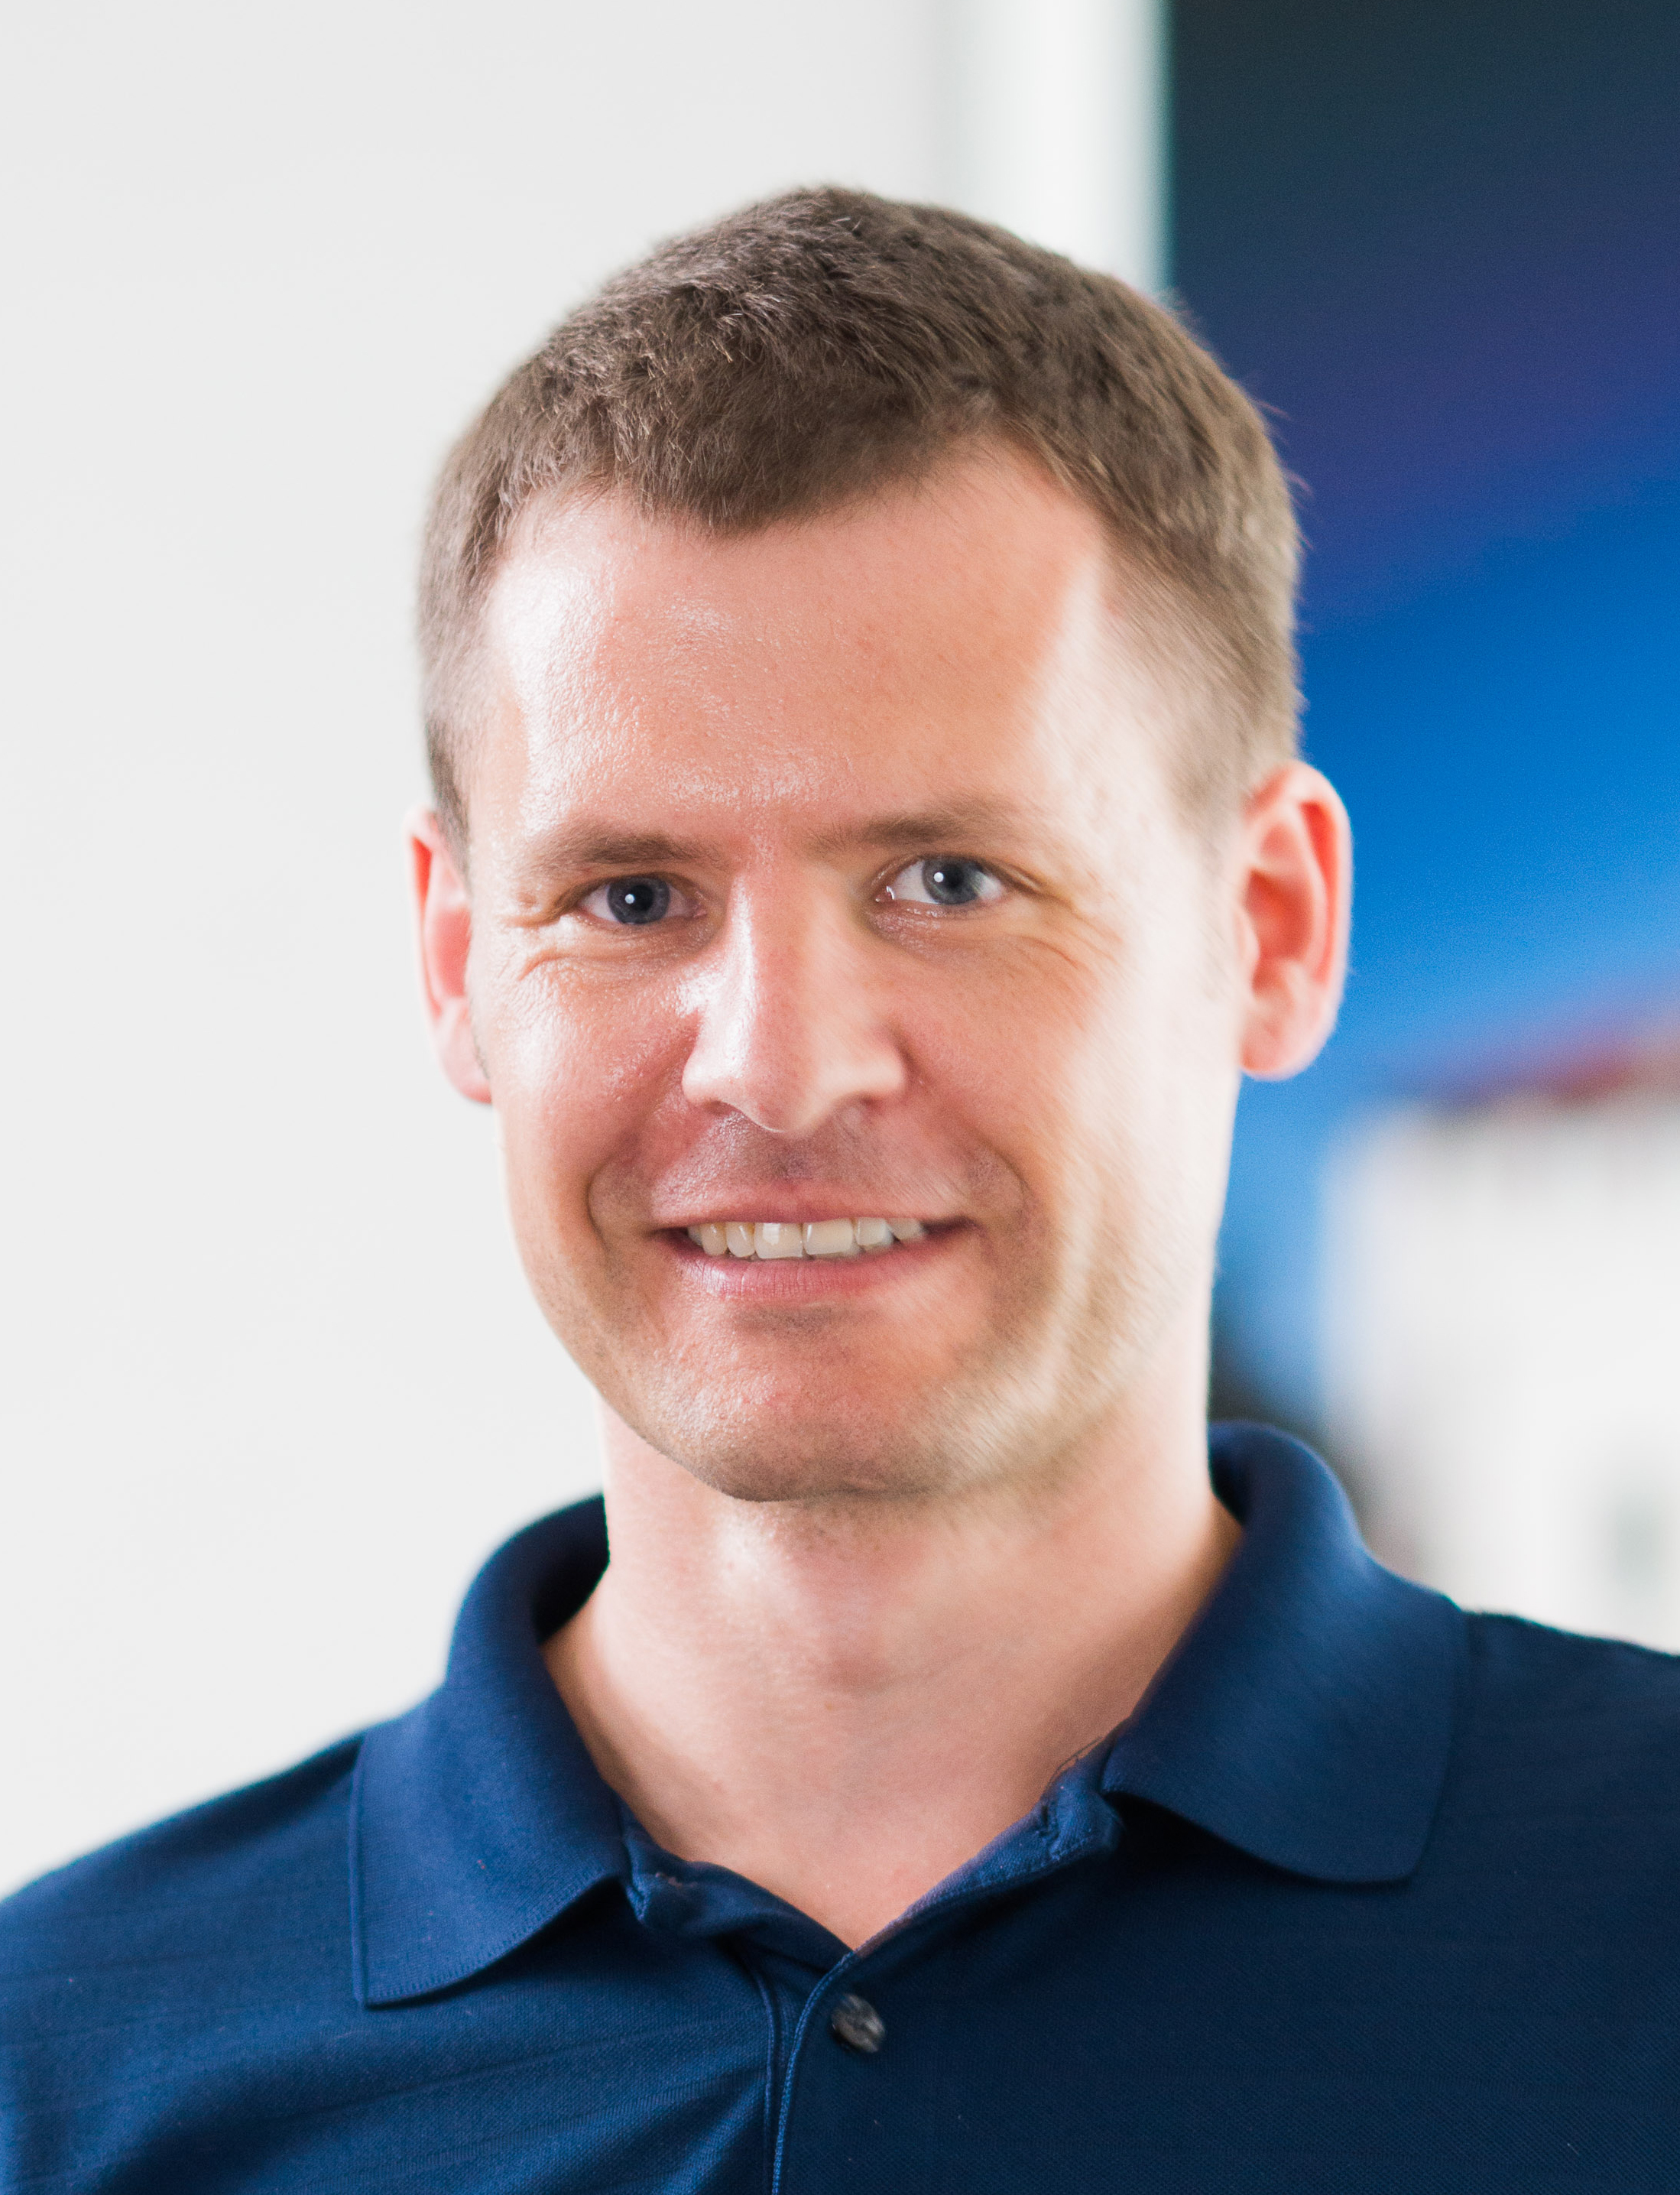
\includegraphics[width=0.9\columnwidth]{res/vorstellungsfotos/wolfram_pernice.jpg}\\
\smallskip
Prof.\ Dr.\ Wolfram\ Pernice\\
Physikalisches Institut
\end{center}

Zusammen mit meinem Kollegen Prof.\ Dr.\ Stefan\ Linz werde ich Sie in den kommenden drei Semestern im Integrierten Kurs (Physik 1-3) näher kennenlernen. Wir halten den Kurs zusammen nun zum zweiten Mal und ich hoffe Sie in den nächsten Semestern für die Experimentalphysik begeistern zu können.

Meine Arbeitsgruppe am Physikalischen Institut und am CeNTech untersucht optische Nanostrukturen. Wir stellen integrierte Chips im Reinraum mit modernen Methoden der Nanofertigung her und untersuchen deren Eigenschaften mit Präzisionsmessungen, aber auch mit einer Reihe von Simulationsmethoden. Ein langfristiges Ziel dabei ist die Realisierung optischer Quantencomputer, sowie die abhörsichere Kommunikation mit einzelnen Lichtquanten und die schnelle Datenverarbeitung. Wenn Sie gerne mit Licht und Lasern spielen sind Sie bei uns genau richtig (und können auch gerne einmal im Labor vorbei schauen). Vielleicht entscheiden Sie sich ja auch später für eine Bachelor- oder Masterarbeit auf dieser Thematik.

Mein Weg in die Physik begann in den Ingenieurwissenschaften mit einem Studium der Mikrosystemtechnik an der Universität Freiburg (1998-2004). Nach einem Auslandsjahr (was ich Ihnen jetzt schon sehr empfehlen kann) in den USA an der Indiana University in Bloomington promovierte ich an der University of Oxford, diesmal im Bereich angewandte Mathematik und Elektrotechnik (von 2004-2007). Als Humboldt-Stipendiat verbrachte ich knapp 4 Jahre an der Yale University wo ich mich mit nanophotonischen Strukturen und optischen Messmethoden befasste. Vor meiner Berufung an die WWU Anfang 2015 leitete ich eine Nachwuchsgruppe am Karlsruher Institut für Technologie, im Bereich der integrierten Quantenoptik und Optomechanik.

Ein breites Fächerspektrum hat sich für mich in Retrospektive sehr bewährt, daher möchte ich auch versuchen Ihnen die vielen Facetten der Physik und verwandter Fächer in ihrer Breite näher zu bringen. Ich wünsche Ihnen dazu einen erfolgreichen Start und viel Freude beim Studium der Physik.


\includegraphics[width=\columnwidth]{res/pernice_illustration.jpg}
\end{multicols}

\newpage

\begin{multicols}{2}
\begin{center}
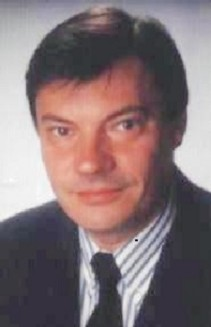
\includegraphics[width=0.71\columnwidth]{res/vorstellungsfotos/linz.jpg}\\
Prof.\ Dr.\ Stefan\ J.\ Linz\\
Institut für Theoretische Physik
\end{center}

Ich freue mich darauf, in den nächsten drei Semestern den theoretischen Teil des Integrierten Kurses zu lesen. Dabei möchte ich Ihnen nicht nur die theoretischen Grundlagen der Klassischen Physik vermitteln, sondern Sie auch in die grundlegenden Konzepte und Denkweisen der
theoretischen Physik einführen und Ihnen die Effektivität und Eleganz einer mathematisch formulierten Naturbeschreibung näher bringen. Meine Grundausbildung als Physiker habe ich an der Universität des Saarlandes in Saarbrücken erhalten und dort auch 1989 promoviert. Daran schloss sich ein mehrjähriger Auslandsaufenthalt in den USA an, als Postdoctoral Fellow bei der Woods Hole Oceanographic Institution (WHOI) und danach als Research Associate im Department of Applied Mathematics der Northwestern University in Evanston bei Chicago. Nach Rückkehr nach Deutschland arbeitete ich als wissenschaftlicher Assistent, später als Oberassistent im Institut für Physik an der Universität Augsburg, wo ich mich 1997 habilitierte und zum Privatdozenten ernannt wurde. 2002 folgte ich einem Ruf auf eine Professur für Theoretische Physik an der WWU Münster.

Forschungsschwerpunkt meiner Arbeitsgruppe ist Theorie komplexer Systeme, insbesondere die Modellierung und theoretische Analyse zeitlicher bzw.\ raumzeitlicher Dynamik in Systemen, die spontan durch das Wechselspiel von Nichtgleichgewicht, Nichtlinearität und Dissipation entstehen kann. Physikalisch stehen dabei Depositions- und Erosionsphänomene, die Dynamik granularer Materie und komplexer Fluide sowie mathematische Aspekte der Theorie chaotischer Systeme im Vordergrund.

\begin{center}
\includegraphics[width=0.7\columnwidth]{res/comics/manchmal_verbessert.jpg}\\
{\footnotesize 
S. Harris - sciencecartoonsplus.com}
\end{center}
\end{multicols}

\medskip

\begin{center}
	\includegraphics[width=0.7\textwidth]{res/comics/teaching_physics.png}
\end{center}

\newpage

\begin{multicols}{2}
\begin{center}
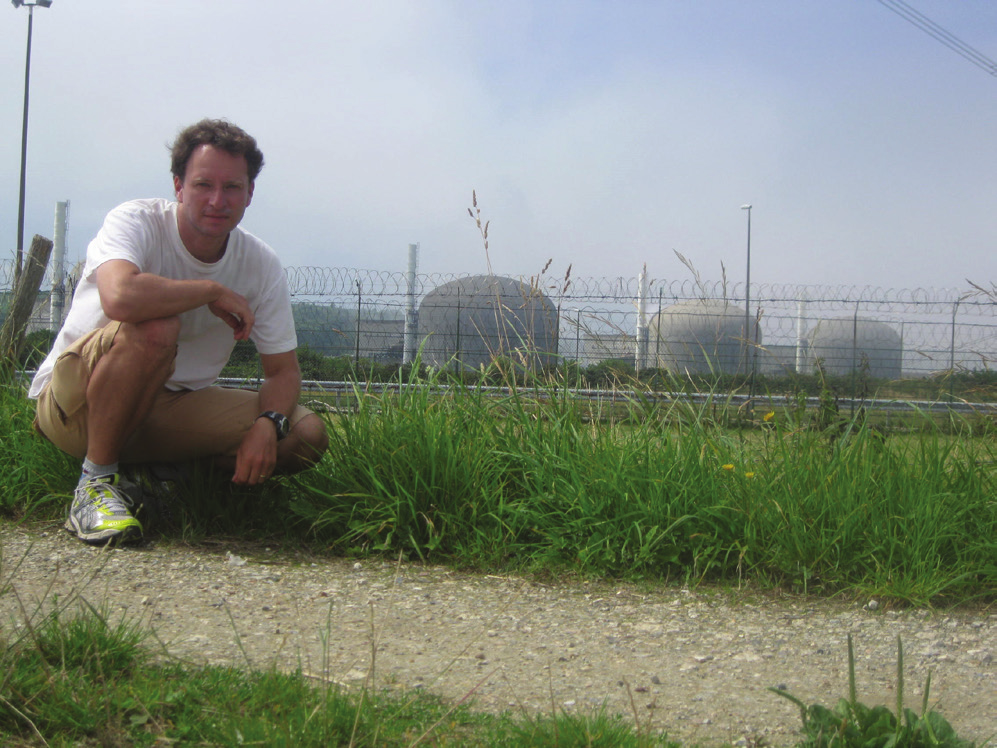
\includegraphics[width=0.9\columnwidth]{res/vorstellungsfotos/wulkenhaar.png}\\
Prof.\ Dr.\ Raimar\ Wulkenhaar\\
Mathematisches Institut
\end{center}

Ich bin von der Ausbildung her Physiker, arbeite im Grenzgebiet zwischen Mathematik und Physik und bin seit 2005 Professor für Reine Mathematik am Fachbereich Mathematik und Informatik der WWU.

Die Vorlesung „Mathematik für Physiker“ wird traditionell vom Mathematischen Institut veranstaltet. Ich selbst werde den Zyklus zum 7. Mal halten. Es ist aus meiner Sicht eine schöne Vorlesung; mir ist aber klar, dass die meisten Studierenden das anders sehen.

Auch wenn der Stoff durchaus umfangreich ist, können wir nur einen kleinen Teil dessen behandeln, was die Physik benötigt. Es geht in der Vorlesung nicht um die Bereitstellung von Rechenwerkzeugen für die Physik; das bekommen Sie nebenbei in den Physikvorlesungen geliefert. Es geht in der Mathematik darum zu verstehen, weshalb diese Rechenwerkzeuge so und nicht anders funktionieren. Der Einstieg in die Denkweise der Mathematik ist für viele nicht leicht. Erst im Lauf der Zeit entsteht rückblickend ein gewisses Verständnis für die tiefliegenden Strukturen und Zusammenhänge der Mathematik. Im Idealfall gelangen Sie so zu einer soliden Grundlage, mit der Sie die Rechenwerkzeuge der Physik nicht nur verstehend nutzen, sondern kreativ weiterentwickeln können.


\[
\resizebox{0.45\hsize}{!}{$\displaystyle\sum_{n = 1}^\infty \frac{1}{n^2} = \frac{\pi^2}{6}$}
\]

Nun noch einige Informationen zu mir. Nach Physikistudium an der Universität Leipzig mit Abschluss als Diplomphysiker. 1994 habe ich in Leipzig auch meine Doktorarbeit geschrieben und 1997 verteidigt. Dabei ging es um die Formulierung von Modellen der Teilchenphysik im Rahmen der nichtkommutativen Geometrie. Die Ergebnisse sind rückblickend völlig unwichtig, sie haben mich aber 1998/1999 als DAAD-Postdoc nach Marseille gebracht.

Ich habe am Centre de Physique Theorique in Marseille mein Arbeitsgebiet gefunden, die Quantenfeldtheorie auf nichtkommutativen Geometrien. Vereinfacht gesagt geht es um die Frage (und ihre Konsequenzen), ob man auf beliebig kleinen Längenskalen, sagen wir $10^{-80}$ m, noch Physik betreiben kann. Es gibt gute Gründe anzunehmen, dass das unmöglich ist, und entsprechend sollte zur Formulierung physikalischer Gesetze eine Geometrie benutzt werden, in der $10^{-80}$ m ebenfalls sinnlos sind. Diese Nichtkommutative Geometrie wird in einer Sprache analog zur Quantenphysik beschrieben.

Seit Marseille, vor allem aber seit meiner zweiten Postdoc-Station 2000/2001 an der Universität Wien, arbeite ich an quantenfeldtheoretischen Modellen auf einer besonders einfachen nichtkommutativen Geometrie. Während meines dritten Postdoc-Aufenthalts 2002/2005 am Max- Planck-Institut für Mathematik in den Naturwissenschaften in Leipzig konnte ich mit meinem Kollegen aus Wien zusammen eine größere Hürde beseitigen. Die mathematisch rigorose Konstruktion einer 4-dimensionalen Quantenfeldtheorie auf einer nichtkommutativen Geometrie konnten wir inzwischen abschließen. Etwas analoges ist in der üblichen kommutativen Geometrie bisher nicht geglückt. Es resultierten spannende Fragen, an denen ich seitdem arbeite.

\begin{center}
\includegraphics[width=0.85\columnwidth]{res/comics/calvin_mathe.png}
\end{center}
\end{multicols}
